% Chapter 4

\chapter{Methodology and Evaluation Protocol}
\label{Chapter4}
\lhead{Chapter 4. \emph{Methodology and Evaluation Protocol}}

\section{Experimental Design}
The evaluation is designed to allow for the independent measurement of three
claims; namely utility, security and systems performance. The utility aspects are
evaluated by comparing agents that must author task logic inline against agents
that can register and reuse that logic as a dynamic tool. The security aspects are tested through
attempting to breach containment generated by the use of an adversarially
created codebase. Finally, the performance characteristics of moving the
execution point of a process-level sandbox into a Firecracker microVM are
measured. Figure 4.1 describes the three independent evaluation axes used in the
evaluation.

\begin{figure}[htbp]
    \centering
    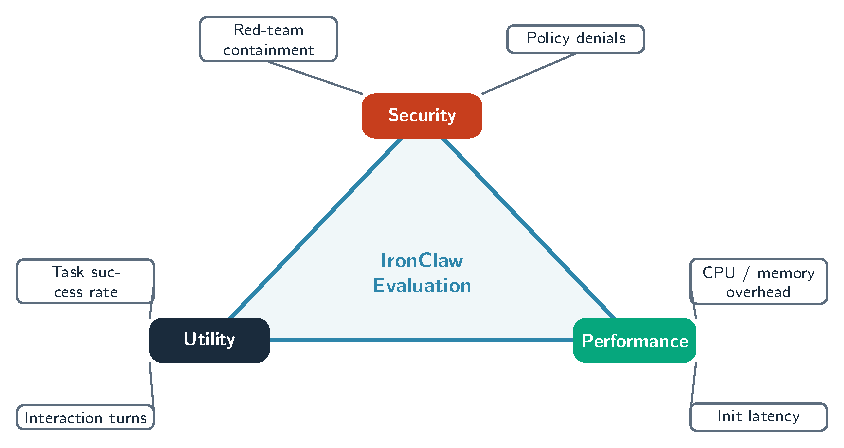
\includegraphics[width=0.85\linewidth]{Figures/fig_evaluation_pillars.pdf}
    \caption{Evaluation methodology overview: utility, security, and performance experiments are run independently and together answer the thesis research questions.}
    \label{fig:evaluation_pillars}
\end{figure}

\section{Baselines}
The two hypotheses require different matched baselines.

\noindent\textbf{H1 baseline:} an agent with generic SQL or sandboxed-script
capabilities that must author the required task logic inline for every request.
The H1 target receives the same capabilities plus runtime tool registration and
an explicit reuse policy.

\noindent\textbf{H2 baseline:} an ordinary child process executing the same
generated shell payload with the invoking user's view of host resources. The H2
target executes that payload inside IronClaw's Firecracker guest through the
authenticated vsock tool path.

\section{Utility and Security Evaluation}
Utility is evaluated using deterministic SQL, legacy-parser, and repository
compliance tasks. Metrics include answer correctness, model steps,
tool calls, billed input and output tokens, reasoning tokens, authored code, and
wall-clock time. Repetitive and mixed workloads isolate whether the one-time
creation cost is amortized.

Security is evaluated with five non-destructive host-resource attacks covering
file confidentiality, file integrity, environment confidentiality, device
visibility, and process-namespace visibility. A payload is contained only when
the targeted host resource remains unobserved and unmodified. The acceptance
criterion is zero successful accesses in the microVM condition.

\begin{figure}[htbp]
    \centering
    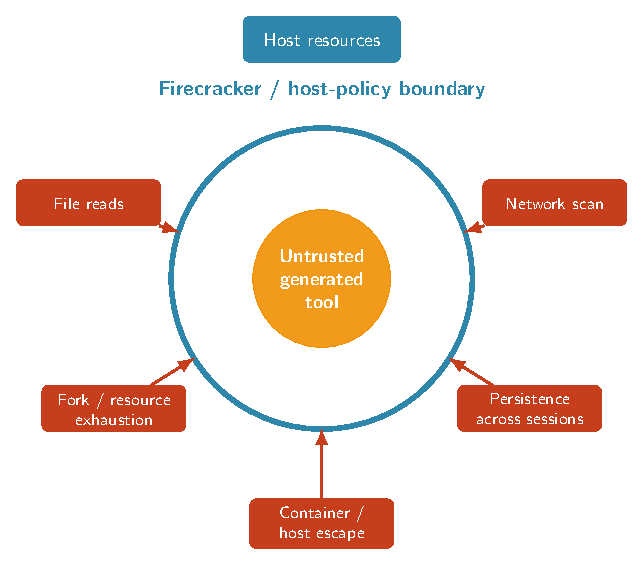
\includegraphics[width=0.9\linewidth]{Figures/fig_threat_model.pdf}
    \caption{Containment boundary for malicious synthesized tools. Attack vectors are blocked by the Firecracker and host-policy boundary.}
    \label{fig:threat_model}
\end{figure}

\fref{fig:threat_model} illustrates the containment boundary that the red-team
suite is designed to test.

\section{Performance Profiling}
Performance profiling measures:
\begin{itemize}
    \item process creation and microVM cold initialization latency;
    \item warm guest execution latency over an authenticated vsock session;
    \item host resident memory and configured guest memory;
    \item CPU time and utilization for a bounded workload; and
    \item stop, restart, authentication, and successful-probe recovery time.
\end{itemize}

The initialization target is $<500$\,ms for snapshot-resumed guests. Cold boot is
reported separately and does not test that target. Ten cold starts, twenty warm
executions, and five recovery trials are used in Chapter~\ref{ChapterH2}.

\begin{figure}[htbp]
    \centering
    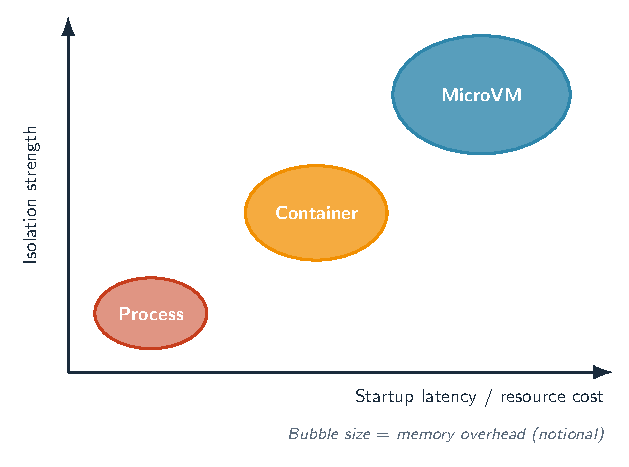
\includegraphics[width=0.85\linewidth]{Figures/fig_sandbox_comparison.pdf}
    \caption{Conceptual trade-off between isolation strength and runtime cost across the three execution modes compared in this thesis.}
    \label{fig:sandbox_comparison}
\end{figure}

Figure 4.3 shows how a tradeoff between Isolation Strength and Runtime Cost can
be expected.
